\documentclass[12pt,letterpaper]{article}

% Paquetes esenciales para matemáticas y español
\usepackage[utf8]{inputenc}
\usepackage[spanish,es-tabla]{babel}
\usepackage{amsmath}
\usepackage{amsfonts}
\usepackage{amssymb}
\usepackage{geometry}
\usepackage{verbatim}
\usepackage{graphicx}
\usepackage{float}
\usepackage{subcaption} 
\usepackage{tikz}

% Configuración de los márgenes
\geometry{left=2.5cm, right=2.5cm, top=2.5cm, bottom=2.5cm}

\begin{document}
	
	\begin{center}
		\Large \textbf{METROLOGÍA ÓPTICA} \\
		\vspace{0.3cm}
		\large \textbf{TAREA 3}
	\end{center}
	
	\vspace{0.5cm}
	\noindent \textbf{NOMBRE:} \underline{Jonathan Francisco Rojas Martínez} \hfill \textbf{FECHA:} \underline{7 de julio de 2026}
	
	\vspace{0.5cm}
	\noindent \textbf{INSTRUCCIONES.-} Conteste de manera completa las siguientes preguntas.
	\vspace{0.5cm}
	
	\begin{enumerate}
		\item[1.-] ¿Defina interferometría de medición de fase y qué técnicas/métodos existen?
		
		\vspace{0.3cm}
		\textbf{Respuesta:} \\
		La interferometría de medición de fase (Phase-Shifting Interferometry, PSI) es una técnica metrológica de alta precisión utilizada para reconstruir la topografía o el mapa de fase óptica de un frente de onda. Consiste en registrar una serie de patrones de interferencia (interferogramas) mientras se introduce un cambio de fase conocido y controlado entre el haz de prueba y el haz de referencia. A partir de estas variaciones de intensidad, es posible recuperar la fase de forma unívoca en cada píxel.
		
		Entre las principales técnicas y métodos existentes se encuentran:
		\begin{itemize}
			\item \textbf{Métodos Temporales (Temporal Phase Shifting):} Introducen el desfase de manera secuencial en el tiempo utilizando un actuador piezoeléctrico (PZT). Ejemplos: métodos de 3, 4 o 5 pasos, algoritmos de Carré y Hariharan.
			\item \textbf{Métodos Espaciales (Spatial Phase Shifting):} Introducen múltiples desfases simultáneamente en diferentes regiones del espacio o en sensores multiplexados, permitiendo mediciones en tiempo real (dinámicas).
			\item \textbf{Demodulación Espacial por Transformada de Fourier (Método de Takeda):} Requiere un único interferograma que contenga una portadora espacial de alta frecuencia, separando las componentes en el dominio espectral.
		\end{itemize}
		\vspace{0.5cm}
		
		\item[2.-] Describa la teoría básica del método de \textit{phase stepping} para obtener la fase óptica.
		
		\vspace{0.3cm}
		\textbf{Respuesta:} \\
		El método de \textit{phase stepping} consiste en variar de forma discreta y controlada la fase del haz de referencia en pasos sucesivos $\alpha_i$. La intensidad registrada por un detector en un punto $(x,y)$ para el paso $i$-ésimo se expresa mediante la ecuación fundamental de la interferometría:
		\[ I_i(x,y) = I_{dc}(x,y) + I_{ac}(x,y) \cos(\phi(x,y) + \alpha_i) \]
		Donde las tres incógnitas principales a resolver por cada píxel son:
		\begin{enumerate}
			\item $I_{dc}(x,y)$: Intensidad de fondo o componente de corriente continua (Background intensity).
			\item $I_{ac}(x,y)$: Amplitud de modulación de las franjas (Fringe visibility).
			\item $\phi(x,y)$: La fase óptica del objeto que se desea medir.
		\end{enumerate}
		Dado que hay tres parámetros desconocidos, se requiere capturar un mínimo de $N \ge 3$ imágenes con diferentes desfases conocidos $\alpha_i$ para plantear un sistema de ecuaciones resoluble que permita aislar matemáticamente la fase $\phi(x,y)$ mediante funciones trigonométricas inversas.
		\vspace{0.5cm}
		
		\item[3.-] Encuentre $\Delta\theta$ para un algoritmo de 3 pasos, con paso de $\alpha = (\pi/4, 3\pi/4 \text{ y } 5\pi/4)$.
		
		\vspace{0.3cm}
		\textbf{Respuesta:} \\
		Denotemos la fase de interés como $\phi$ (equivalente a $\Delta\theta$). Las tres ecuaciones de intensidad correspondientes a los desfases propuestos son:
		\[ I_1 = I_{dc} + I_{ac} \cos\left(\phi + \frac{\pi}{4}\right) \]
		\[ I_2 = I_{dc} + I_{ac} \cos\left(\phi + \frac{3\pi}{4}\right) \]
		\[ I_3 = I_{dc} + I_{ac} \cos\left(\phi + \frac{5\pi}{4}\right) \]
		Desarrollando los términos de coseno mediante identidades trigonométricas de adición:
		\[ \cos\left(\phi + \frac{\pi}{4}\right) = \frac{\sqrt{2}}{2}(\cos\phi - \sin\phi) \]
		\[ \cos\left(\phi + \frac{3\pi}{4}\right) = \frac{\sqrt{2}}{2}(-\cos\phi - \sin\phi) \]
		\[ \cos\left(\phi + \frac{5\pi}{4}\right) = \frac{\sqrt{2}}{2}(-\cos\phi + \sin\phi) \]
		Sustituyendo estos desarrollos en el sistema original:
		\[ I_1 = I_{dc} + I_{ac} \frac{\sqrt{2}}{2}(\cos\phi - \sin\phi) \]
		\[ I_2 = I_{dc} + I_{ac} \frac{\sqrt{2}}{2}(-\cos\phi - \sin\phi) \]
		\[ I_3 = I_{dc} + I_{ac} \frac{\sqrt{2}}{2}(-\cos\phi + \sin\phi) \]
		Para eliminar la componente de fondo $I_{dc}$, realizamos las diferencias entre las intensidades:
		\[ I_1 - I_2 = I_{ac} \frac{\sqrt{2}}{2} \left[ (\cos\phi - \sin\phi) - (-\cos\phi - \sin\phi) \right] = \sqrt{2} I_{ac} \cos\phi \]
		\[ I_3 - I_2 = I_{ac} \frac{\sqrt{2}}{2} \left[ (-\cos\phi + \sin\phi) - (-\cos\phi - \sin\phi) \right] = \sqrt{2} I_{ac} \sin\phi \]
		Dividiendo la segunda diferencia entre la primera para eliminar el factor de modulación $\sqrt{2}I_{ac}$:
		\[ \frac{I_3 - I_2}{I_1 - I_2} = \frac{\sqrt{2} I_{ac} \sin\phi}{\sqrt{2} I_{ac} \cos\phi} = \tan\phi \]
		Por lo tanto, la fase $\Delta\theta$ buscada es de la forma:
		\[ \Delta\theta = \arctan\left(\frac{I_3 - I_2}{I_1 - I_2}\right) \]
		\vspace{0.5cm}
		
		\item[4.-] Programe las ecuaciones de Intensidad para un algoritmo de 3 pasos y encuentre $\Delta\theta$. Envíe el programa y los resultados.
		
		\vspace{0.3cm}
		\textbf{Respuesta:} \\
		A continuación se presenta el código desarrollado en Python utilizando librerías estándar para simular la generación de los tres interferogramas y reconstruir con éxito la fase original mediante la fórmula deducida.
		
		\begin{verbatim}
			import numpy as np
			
			# 1. Definición de parámetros espaciales y fase sintética
			x = np.linspace(-5, 5, 500)
			X, Y = np.meshgrid(x, x)
			fase_original = 
			= 2 * np.pi * np.exp(-(X**2 + Y**2)/4) # Fase de prueba (gaussiana)
			
			# Parámetros del interferograma
			I_dc = 1.0  # Intensidad de fondo
			I_ac = 0.8  # Visibilidad de franjas
			
			# 2. Desfases del algoritmo de 3 pasos
			alpha1 = np.pi / 4
			alpha2 = 3 * np.pi / 4
			alpha3 = 5 * np.pi / 4
			
			# 3. Generación de las ecuaciones de intensidad
			I1 = I_dc + I_ac * np.cos(fase_original + alpha1)
			I2 = I_dc + I_ac * np.cos(fase_original + alpha2)
			I3 = I_dc + I_ac * np.cos(fase_original + alpha3)
			
			# 4. Reconstrucción de la fase envolvente (Delta_theta)
			fase_recuperada = np.arctan2(I3 - I2, I1 - I2)
			
			# Verificación de resultados numéricos en el centro de la matriz
			print("Fase original en el centro:", fase_original[250, 250])
			# El resultado de arctan2 está envuelto en el rango [-pi, pi]
			fase_original_wrapped =
			= np.arctan2(np.sin(fase_original), np.cos(fase_original))
			print("Fase recuperada envuelta en el centro:", fase_recuperada[250, 250])
			print("Error absoluto máximo:", 
			np.max(np.abs(fase_original_wrapped - fase_recuperada)))
		\end{verbatim}
		
		\textbf{Resultados de la simulación:} \\
		\begin{figure}
			\centering
			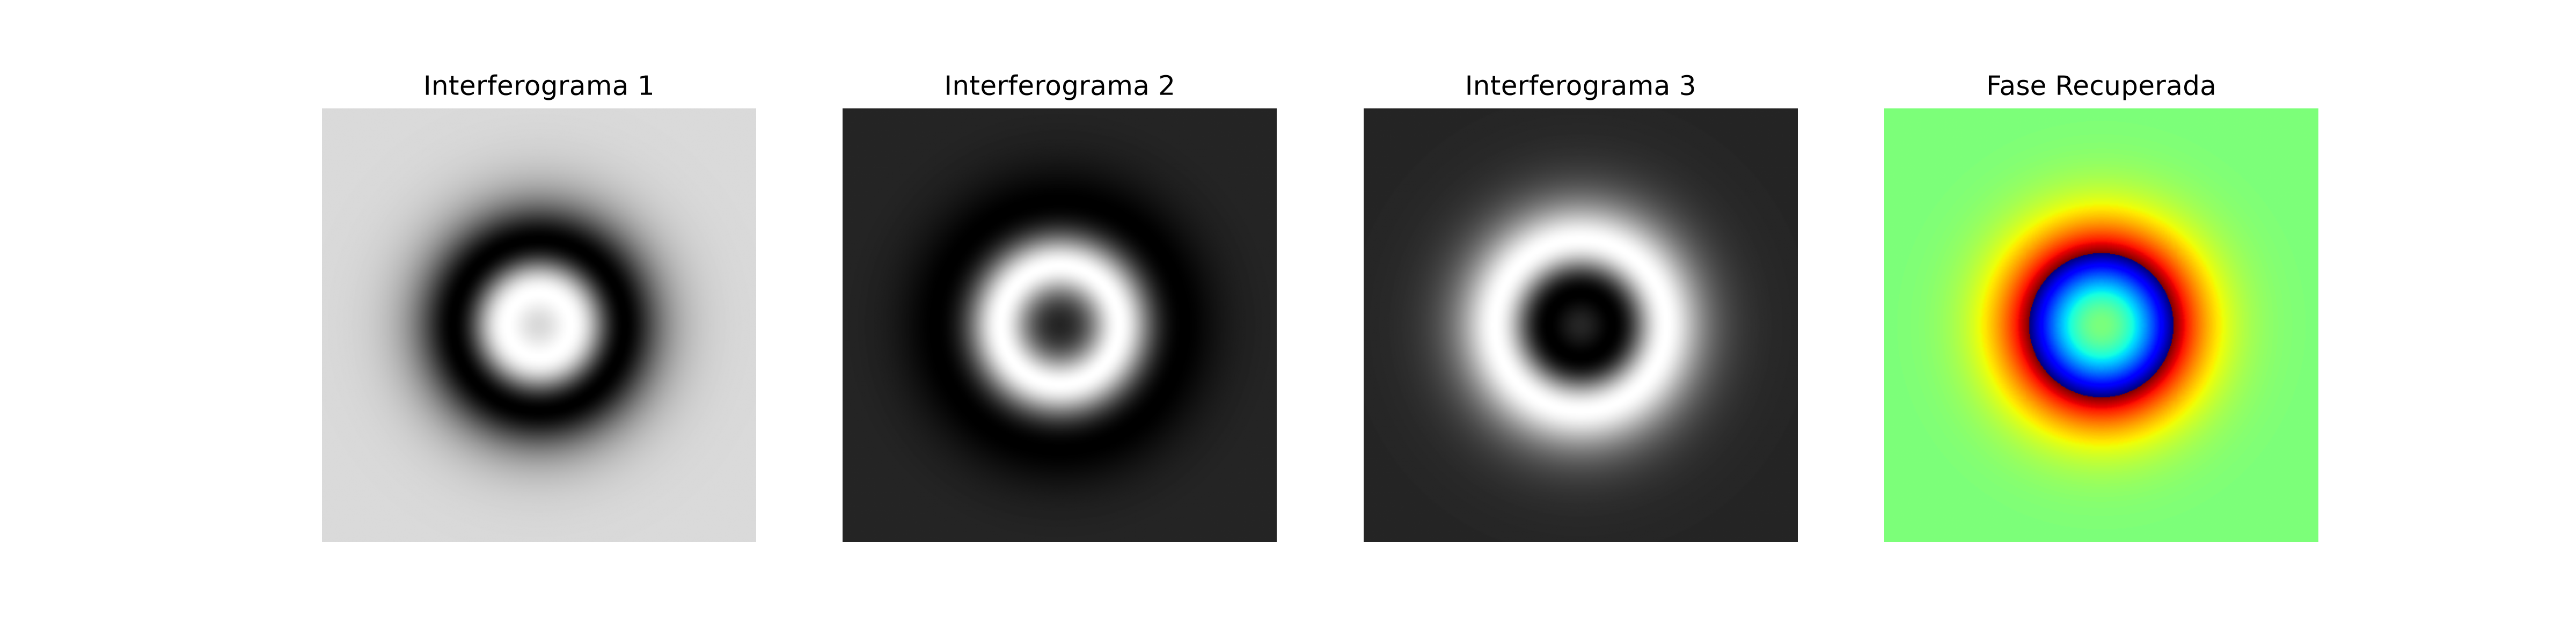
\includegraphics[width=1\linewidth]{resultados.png}
			\caption{Desenvolviendo la fase por el método de 3 pasos.}
			\label{fig:placeholder}
		\end{figure}
			
		
		\item[6.-] Explique, deduzca y describa la utilidad de los algoritmos de Carré y Hariharan.
		
		\vspace{0.3cm}
		\textbf{Respuesta:} \\
		\textbf{Algoritmo de Carré:} \\
		
		Se tienen las siguientes ecuaciones con sus respectivos corrimientos de fase de $2\beta$ entre cada una:
		
		\begin{equation}
			\begin{aligned}
				I_1 &= I' + I''\cos(\phi - 3\beta), \\
				I_2 &= I' + I''\cos(\phi - \beta), \\
				I_3 &= I' + I''\cos(\phi + \beta), \\
				I_4 &= I' + I''\cos(\phi + 3\beta).
			\end{aligned}
		\end{equation}
		
		Ahora se utilizan identidades trigonométricas para reescribir las ecuaciones de la siguiente manera:
		
		\begin{equation}
			\begin{aligned}
				I_1 &= I' + I''(\cos\phi\cos3\beta + \text{sen}\phi\text{sen}3\beta), \\
				I_2 &= I' + I''(\cos\phi\cos\beta + \text{sen}\phi\text{sen}\beta), \\
				I_3 &= I' + I''(\cos\phi\cos\beta - \text{sen}\phi\text{sen}\beta), \\
				I_4 &= I' + I''(\cos\phi\cos3\beta - \text{sen}\phi\text{sen}3\beta).
			\end{aligned}
		\end{equation}
		
		Se elimina la variable $I'$ al calcular las diferencias entre las ecuaciones pares como se indica a continuación:
		
		\begin{equation}
			\begin{aligned}
				I_1 - I_4 &= 2I''\text{sen}\phi\text{sen}3\beta, \\
				I_2 - I_3 &= 2I''\text{sen}\phi\text{sen}\beta.
			\end{aligned}
		\end{equation}
		
		Sustituyendo estos valores en el segundo miembro de la fórmula 2.22 se sigue que:
		
		\begin{equation}
			\frac{3(I_2 - I_3) - (I_1 - I_4)}{(I_1 - I_4) + (I_2 - I_3)} = \frac{6I''\text{sen}\phi\text{sen}3\beta - 2I''\text{sen}\phi\text{sen}3\beta}{2I''\text{sen}\phi\text{sen}3\beta + 2I''\text{sen}\phi\text{sen}\beta}
		\end{equation}
		
		\begin{equation}
			\frac{3(I_2 - I_3) - (I_1 - I_4)}{(I_1 - I_4) + (I_2 - I_3)} = \frac{3\text{sen}\beta - \text{sen}3\beta}{\text{sen}3\beta + \text{sen}\beta}
		\end{equation}
		
		Aquí se reescribe la ecuación anterior utilizando la siguiente identidad:
		
		\begin{equation}
			\begin{aligned}
				\text{sen}3\beta &= \text{sen}(\beta + 2\beta), \\
				&= \text{sen}\beta\cos2\beta + \cos\beta\text{sen}2\beta, \\
				&= \text{sen}\beta(\cos^2\beta - \text{sen}^2\beta) + \cos2\beta\text{sen}\beta\cos\beta, \\
				&= 3\text{sen}\beta\cos^2\beta - \text{sen}^3\beta.
			\end{aligned}
		\end{equation}
		
		Esta expresión nos lleva a:
		
		\begin{equation}
			\frac{3\text{sen}\beta - \text{sen}3\beta}{\text{sen}3\beta + \text{sen}\beta} = \frac{3\text{sen}\beta - 3\text{sen}\beta\cos^2\beta + \text{sen}^3\beta}{3\text{sen}\beta\cos^2\beta - \text{sen}^3\beta + \text{sen}\beta}
		\end{equation}
		
		\begin{equation}
			= \frac{3 - 3\cos^2\beta + \text{sen}^2\beta}{3\cos^2\beta - \text{sen}^2\beta + 1}
		\end{equation}
		
		\begin{equation}
			= \frac{3\text{sen}^2\beta + \text{sen}^2\beta}{3\cos^2\beta + \cos^2\beta}
		\end{equation}
		
		\begin{equation}
			\frac{3(I_2 - I_3) - (I_1 - I_4)}{(I_1 - I_4) + (I_2 - I_3)} = \tan^2\beta
		\end{equation}
		
		Y vemos que este resultado corresponde a lo esperado utilizando el algoritmo de Carré para calcular el corrimiento de fase $\beta$. Para obtener la fase final, se parte de la ecuación 2.23 y se calculan las sumas y diferencias que se encuentran en el segundo miembro de la expresión:
		
		\begin{equation}
			\begin{aligned}
				I_1 - I_4 &= 2I''\text{sen}\phi\text{sen}3\beta, \\
				I_2 - I_3 &= 2I''\text{sen}\phi\text{sen}\beta, \\
				I_1 + I_4 &= 2I' + 2I''\cos\phi\cos3\beta, \\
				I_2 + I_3 &= 2I' + 2I''\cos\phi\cos3\beta.
			\end{aligned}
		\end{equation}
		
		Sustituyendo:
		
		\begin{equation}
			\tan\beta\frac{3(I_1 - I_4) + (I_2 - I_3)}{(I_2 + I_3) - (I_1 + I_4)} = \tan\beta\frac{2I''\text{sen}\phi\text{sen}3\beta + 2I''\text{sen}\phi\text{sen}\beta}{2I' + 2I''\cos\phi\cos\beta - 2I' - 2I''\cos\phi\cos3\beta}
		\end{equation}
		
		\begin{equation}
			= \tan\beta\frac{\text{sen}\phi\text{sen}3\beta + \text{sen}\phi\text{sen}\beta}{\cos\phi\cos\beta - \cos\phi\cos3\beta}
		\end{equation}
		
		\begin{equation}
			= \tan\beta\tan\phi\frac{\text{sen}3\beta + \text{sen}\beta}{\cos\beta - \cos3\beta}
		\end{equation}
		
		Ahora se reescribe la expresión anterior usando la identidad que se presenta a continuación:
		
		\begin{equation}
			\begin{aligned}
				\cos3\beta &= \cos(2\beta + \beta) = \cos2\beta\cos\beta - \text{sen}2\beta\text{sen}\beta, \\
				&= (\cos^2\beta - \text{sen}^2\beta)\cos\beta - 2\text{sen}^2\beta\cos\beta, \\
				&= \cos^3\beta - 3\text{sen}^2\beta\cos\beta.
			\end{aligned}
		\end{equation}
		
		Se obtiene que:	
		
		\begin{equation}
			\tan\beta\tan\phi\frac{\text{sen}3\beta + \text{sen}\beta}{\cos\beta - \cos3\beta} = \tan\phi\tan\beta\frac{3\text{sen}\beta\cos^2\beta - \text{sen}^3\beta + \text{sen}\beta}{\cos\beta - \cos^3\beta + 3\text{sen}^2\beta\cos\beta}
		\end{equation}
		
		\begin{equation}
			\tan\beta\tan\phi\frac{\text{sen}3\beta + \text{sen}\beta}{\cos\beta - \cos3\beta} = \tan\phi\tan^2\beta\frac{3\cos^2\beta - \text{sen}^2\beta + 1}{1 - \cos^2\beta + 3\text{sen}^2\beta}
		\end{equation}
		
		\begin{equation}
			= \tan\phi\tan^2\beta\frac{1}{\tan^2\beta}
		\end{equation}
		
		Lo que nos lleva a la expresión esperada para calcular la fase $\phi$ mediante el algoritmo de Carré:
		
		\begin{equation}
			\tan\phi = \frac{3(I_1 - I_4) + (I_2 - I_3)}{(I_2 + I_3) - (I_1 + I_4)}
		\end{equation}
		
		
		\vspace{0.2cm}
		\textbf{Algoritmo de Hariharan (5 pasos):} \\
		Utiliza 5 capturas simétricas distribuidas con un desfase nominal de $\alpha = \pi/2$, tomando los valores de $\{- \pi, -\pi/2, 0, \pi/2, \pi\}$. La fase se calcula mediante la relación canónica:
		\[ \tan\phi = \frac{2(I_2 - I_4)}{2I_3 - I_1 - I_5} \]
		\textit{Utilidad:} Su importancia crítica reside en que es altamente insensible a errores lineales de calibración del PZT. Si existe un desajuste sistemático, el error inducido en el cálculo final se cancela en primer orden, convirtiéndolo en uno de los algoritmos estándares de la industria metrológica por su alta robustez.
		\vspace{0.5cm}
		
		\item[7.-] Encuentre la fase óptica para el algoritmo de Carré para un cambio de fase desconocido.
		
		\vspace{0.3cm}
		\textbf{Respuesta:} \\
		Planteamos las cuatro ecuaciones de intensidad con desfase simétrico desconocido $\alpha$:
		\[ I_1 = I_{dc} + I_{ac} \cos(\phi - 3\alpha/2) \]
		\[ I_2 = I_{dc} + I_{ac} \cos(\phi - \alpha/2) \]
		\[ I_3 = I_{dc} + I_{ac} \cos(\phi + \alpha/2) \]
		\[ I_4 = I_{dc} + I_{ac} \cos(\phi + 3\alpha/2) \]
		Restando los pares externos e internos para suprimir el término continuo $I_{dc}$:
		\[ I_1 - I_4 = 2 I_{ac} \sin\phi \sin(3\alpha/2) \]
		\[ I_2 - I_3 = 2 I_{ac} \sin\phi \sin(\alpha/2) \]
		Sumando los términos respectivos para anular la dependencia de seno de la fase:
		\[ I_2 + I_3 = 2 I_{dc} + 2 I_{ac} \cos\phi \cos(\alpha/2) \]
		\[ I_1 + I_4 = 2 I_{dc} + 2 I_{ac} \cos\phi \cos(3\alpha/2) \]
		Utilizando la identidad trigonométrica del ángulo triple para el cociente de las diferencias:
		\[ \frac{I_1 - I_4}{I_2 - I_3} = \frac{\sin(3\alpha/2)}{\sin(\alpha/2)} = 4\cos^2(\alpha/2) - 1 \]
		De esta expresión despejamos de forma directa la magnitud del desfase desconocido $\alpha$:
		\[ \tan^2\left(\frac{\alpha}{2}\right) = \frac{3(I_2 - I_3) - (I_1 - I_4)}{(I_2 - I_3) + (I_1 - I_4)} \]
		Por otra parte, combinando las sumas para eliminar por completo $I_{dc}$:
		\[ (I_2 + I_3) - (I_1 + I_4) = 4 I_{ac} \cos\phi \cos(\alpha/2) \sin^2(\alpha/2) \]
		Dividiendo de manera adecuada las expresiones obtenidas y sustituyendo el valor hallado para el desfase desconocido $\alpha$, se llega a la célebre ecuación de Carré para la fase óptica:
		\[ \tan\phi = \frac{\sqrt{[(I_1 - I_4) + (I_2 - I_3)][3(I_2 - I_3) - (I_1 - I_4)]}}{I_2 + I_3 - I_1 - I_4} \]
		\vspace{0.5cm}
		
		\item[8.-] Describa claramente el método de demodulación espacial (Método de transformada de Fourier).
		
		\vspace{0.3cm}
		\textbf{Respuesta:} \\
		El método de Transformada de Fourier Espacial (desarrollado originalmente por Takeda) permite extraer la fase óptica de un objeto utilizando \textbf{un único interferograma}. Para lograrlo, se introduce intencionalmente una portadora espacial de alta frecuencia angular $f_0$ mediante la inclinación física de uno de los espejos del interferómetro. El modelo matemático de la intensidad de la imagen capturada es:
		\[ I(x,y) = a(x,y) + b(x,y) \cos(2\pi f_0 x + \phi(x,y)) \]
		Aplicando la identidad de Euler, el interferograma se puede reescribir de forma exponencial compleja:
		\[ I(x,y) = a(x,y) + c(x,y)e^{i 2\pi f_0 x} + c^*(x,y)e^{-i 2\pi f_0 x} \]
		Donde la función compleja de interés que codifica la fase es:
		\[ c(x,y) = \frac{1}{2}b(x,y)e^{i\phi(x,y)} \]
		Al aplicar la Transformada de Fourier unidimensional con respecto al eje espacial $x$, se obtiene en el dominio de la frecuencia:
		\[ \mathcal{F}\{I\}(f_x, y) = A(f_x, y) + C(f_x - f_0, y) + C^*(-f_x - f_0, y) \]
		Debido a la presencia de la frecuencia portadora $f_0$, el espectro se divide nítidamente en tres lóbulos separados en el espacio de frecuencias: la componente espectral de fondo $A(f_x, y)$ centrada en el origen, y las dos bandas laterales de modulación $C$ y $C^*$ desplazadas simétricamente a $+f_0$ y $-f_0$, respectivamente.
		\vspace{0.5cm}
		
		\item[9.-] Encuentre la fase óptica usando el método FFT (Takeda).
		
		\vspace{0.3cm}
		\textbf{Respuesta:} \\
		Continuando con el desarrollo formal planteado en la pregunta anterior, el procedimiento analítico secuencial para aislar y resolver la fase óptica mediante FFT consta de los siguientes pasos:
		\begin{enumerate}
			\item \textbf{Filtrado en Frecuencia:} Se aplica un filtro de ventana pasa-bandas para aislar únicamente el lóbulo positivo $C(f_x - f_0, y)$, eliminando por completo el término de fondo $A$ y la banda conjugada $C^*$.
			\item \textbf{Traslación al Origen:} El lóbulo aislado se desplaza horizontalmente en una magnitud exacta de $-f_0$ hacia el origen de coordenadas espectrales. Este proceso elimina matemáticamente la contribución oscilatoria de la portadora espacial, transformando la señal en $C(f_x, y)$.
			\item \textbf{Transformada Inversa:} Se aplica la Transformada de Fourier Inversa ($\mathcal{F}^{-1}$) para retornar al dominio espacial numérico, obteniendo directamente la señal analítica compleja local $c(x,y)$.
			\item \textbf{Cálculo de la Fase:} La fase óptica envuelta $\phi(x,y)$ se extrae calculando el argumento de la función compleja a través de la parte imaginaria y real de la señal:
			\[ \phi(x,y) = \arctan\left( \frac{\text{Im}\{c(x,y)\}}{\text{Re}\{c(x,y)\}} \right) = \text{atan2}(\text{Im}\{c(x,y)\}, \text{Re}\{c(x,y)\}) \]
		\end{enumerate}
		\vspace{0.5cm}
		
		\item[10.-] Deduzca la ecuación para encontrar la $\Delta\theta$.
		
		\vspace{0.3cm}
		\textbf{Respuesta:} \\
		Para deducir la ecuación general para encontrar la fase $\Delta\theta$ en un esquema general de mínimos cuadrados de $N$ pasos, partimos del modelo analítico de la intensidad:
		\[ I_i = I_{dc} + I_{ac}\cos(\phi + \alpha_i) = I_{dc} + I_{ac}\cos\phi\cos\alpha_i - I_{ac}\sin\phi\sin\alpha_i \]
		Definiendo los coeficientes lineales del sistema:
		\[ a_0 = I_{dc}, \quad a_1 = I_{ac}\cos\phi, \quad a_2 = -I_{ac}\sin\phi \]
		De este modo, la intensidad para cada paso se reduce a la combinación lineal:
		\[ I_i = a_0 + a_1\cos\alpha_i + a_2\sin\alpha_i \]
		Para hallar las estimaciones óptimas de los parámetros ante la presencia de ruido, minimizamos la función de error cuadrático ordinario:
		\[ E(a_0, a_1, a_2) = \sum_{i=1}^N (I_i - a_0 - a_1\cos\alpha_i - a_2\sin\alpha_i)^2 \]
		Calculando las derivadas parciales con respecto a los parámetros $a_1$ y $a_2$, e igualando a cero bajo la condición canónica síncrona donde los desfases cubren uniformemente un ciclo completo ($\sum\cos\alpha_i = \sum\sin\alpha_i = \sum\cos\alpha_i\sin\alpha_i = 0$), las soluciones normales se simplifican a:
		\[ a_1 = \frac{2}{N}\sum_{i=1}^N I_i\cos\alpha_i \]
		\[ a_2 = \frac{2}{N}\sum_{i=1}^N I_i\sin\alpha_i \]
		Finalmente, por definición trigonométrica, conocemos que:
		\[ \tan\phi = \frac{\sin\phi}{\cos\phi} = \frac{-a_2}{a_1} = \frac{\sum_{i=1}^N I_i\sin\alpha_i}{\sum_{i=1}^N I_i\cos\alpha_i} \]
		Por consiguiente, la ecuación analítica universal deducida para encontrar $\Delta\theta$ (o $\phi$) es:
		\[ \Delta\theta = \arctan\left( \frac{\sum_{i=1}^N I_i\sin\alpha_i}{\sum_{i=1}^N I_i\cos\alpha_i} \right) \]
		
	\end{enumerate}
	
\end{document}
